%!TEX root = ../main/main.tex
\section{Overview} % (fold)
\label{sec:overview}
\textbf{myTaxiService} is a taxi service that will operate in a big city; the main purpose is to simplify the access of passengers to the service and to guarantee a fair management of the taxi queues.\\\\
The main stakeholders of the system are the \emph{Users}, the \emph{Taxi Drivers} and the \emph{Operators} as highlighted in \emph{section 1.3} of the \emph{RASD}.\\\\
The system is composed of four main core applications :
\begin{itemize}
	\item Mobile Application (User)
	\item Web Application
	\item Mobile Application (Taxi Driver)
	\item Back-End Application
\end{itemize}
 as stated in \emph{section 1.2.} of the \emph{RASD}.\\
 It's important to highlight that in this document the design of mobile application is based on the Android platform.\\
 Below is shown a diagram representing a general overview of the system.\\
\newpage
\vfill
\begin{figure}[h!t]
\caption{Overview Diagram}
\label{fig:overview-diagram}
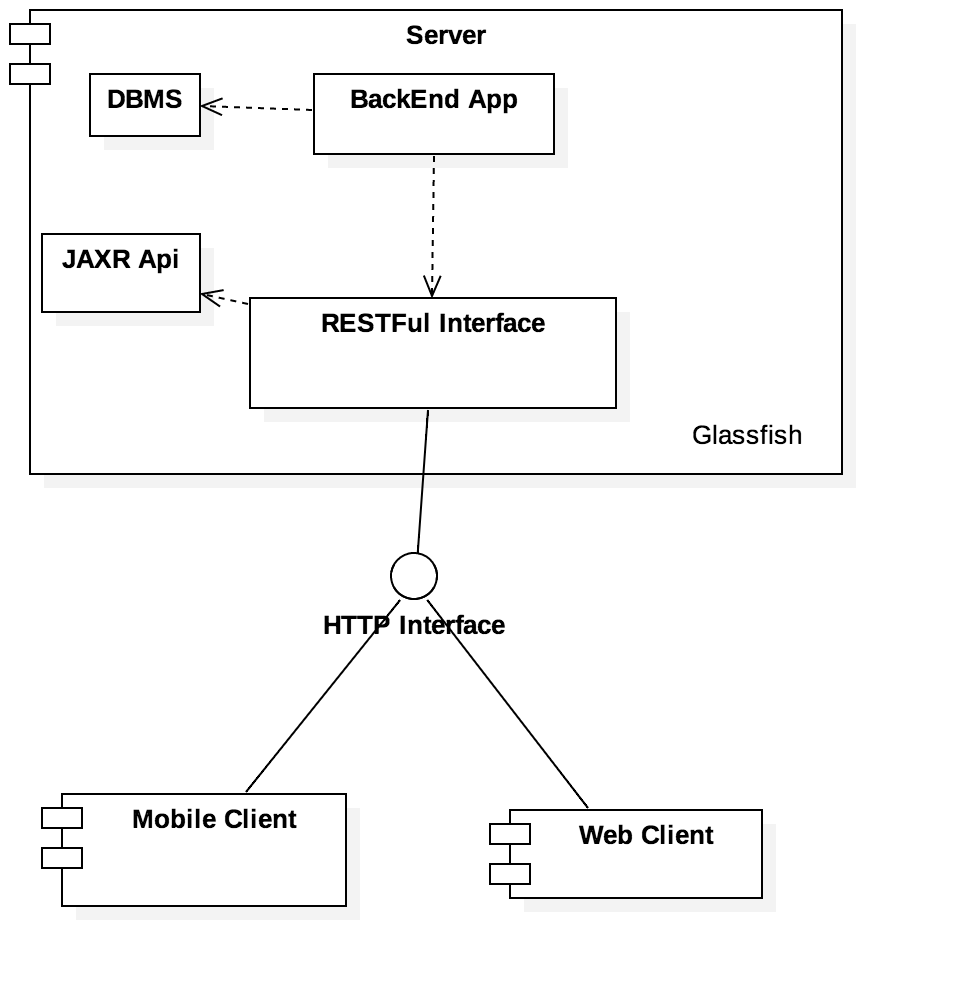
\includegraphics[width=\textwidth]{diagram/png/overview}
\centering
\end{figure}
\vfill
\clearpage

% section overview (end)